%\section{BSM Nonresonant Results}
%\label{sec:nonresonant-results}


In addition to determination of the limit on the SM process, we are
able to provide the results for BSM couplings as described
\ref{sec:nonresMC}.  For the non-resonant signal samples corresponding
to combinations of five anomalous couplings (\kapl. \kapt, \ctwo,
\ctwog, and \cg) listed in Table~\ref{tab:bench_old} (these are also
called "nodes"), the limits are shown on Fig.~\ref{fig:NRlim_nodes}.
The limits for the benchmarks listed in Table~\ref{tab:bench} and
described in Sec.~\ref{sec:nonresMC} are shown in
Fig.~\ref{fig:NRlim_bench}.  Figure~\ref{fig:NRlim_lambda} shows the
``lambda-scan'' - the upper limits for the assumption of changing
$\kappa_\lambda$, while keeping other couplings fixed to their SM
values. Figure~\ref{fig:NRlim_2D} shows a scan over $\lambda-\kappa_t$
parameter space. 
Those results are yet to be updated with the final selection described in that chapter. 
They use a previous version of the categorization procedure, based on the 2015 analysis.

% The $95\%$ CL expected limits are shown as the
% product of the~~\HH~~production cross section and the~\ggbb~~branching
% ratio~~\sigmaHH $\times$ \ggbb, on figure~\ref{fig:BR_limits} together
% with the one and two-$\sigma$ boundaries, for $m_{cat} = 350.~GeV$
% will be updated accordingly).
% Figure~\ref{fig:BR_limits_PlusAll} shows
% in addition, the expected limits when no mass categorization is
% performed. An improvement of the limits between $9.\%$ and $27.\%$ is
% observed.  Table~\ref{tab:mcat} lists the limits and the improvements
% values for each set of anomalous couplings. The improvement reaches
% $24.\%$ for the SM sample. The optimisation of the $m_{cat}$ value has
% been performed with a scan as shown in
% figure~\ref{fig:BR_limits_mScan}. The figure shows the $95\%$ expected
% limits for 4 values of $m_{cat}: 300., 350.,
% 400.,~~and~~450. GeV$. for the 14 nodes. For the SM node (node =1 ),
% $m_{cat} = 350.~GeV$ seems to be the optimal value as for most of the
% other nodes.
% 

\begin{figure*}[h]
  \centering
  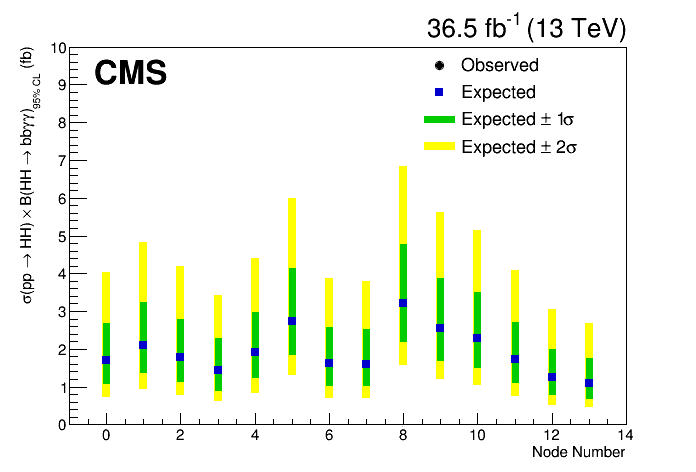
\includegraphics[width=0.8\textwidth]{NR_limits/NR_Limit_Nodes}\hfil
  \caption{Limits for Nodes specified in Table~\ref{tab:bench_old}.}
  \label{fig:NRlim_nodes}
\end{figure*}

\begin{figure*}[h]
  \centering
  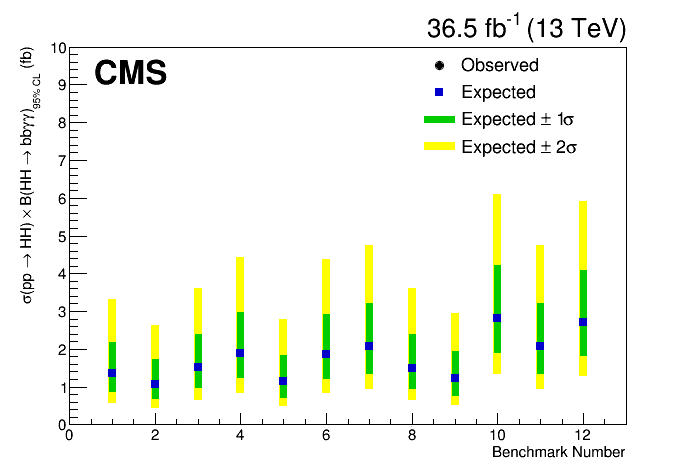
\includegraphics[width=0.8\textwidth]{NR_limits/NR_Limit_Bench}\hfil
  \caption{Limits for Benchmarks described in Sec.~\ref{sec:nonresMC} in Table~\ref{tab:bench}.}
  \label{fig:NRlim_bench}
\end{figure*}


\begin{figure*}[h]
  \centering
  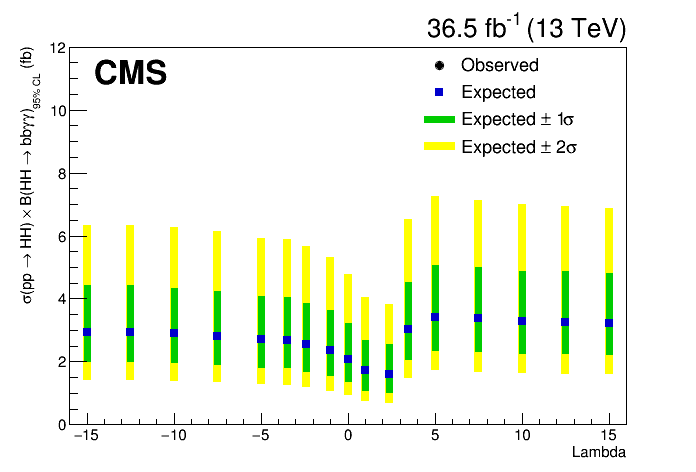
\includegraphics[width=0.8\textwidth]{NR_limits/NR_Limit_LambdaScan}\hfil
  \caption{Upper limits for the BSM models with varying
    $\kappa_\lambda$ parameter, while others fixed to their SM
    values.}
  \label{fig:NRlim_lambda}
\end{figure*}

\begin{figure*}[h]
  \centering
  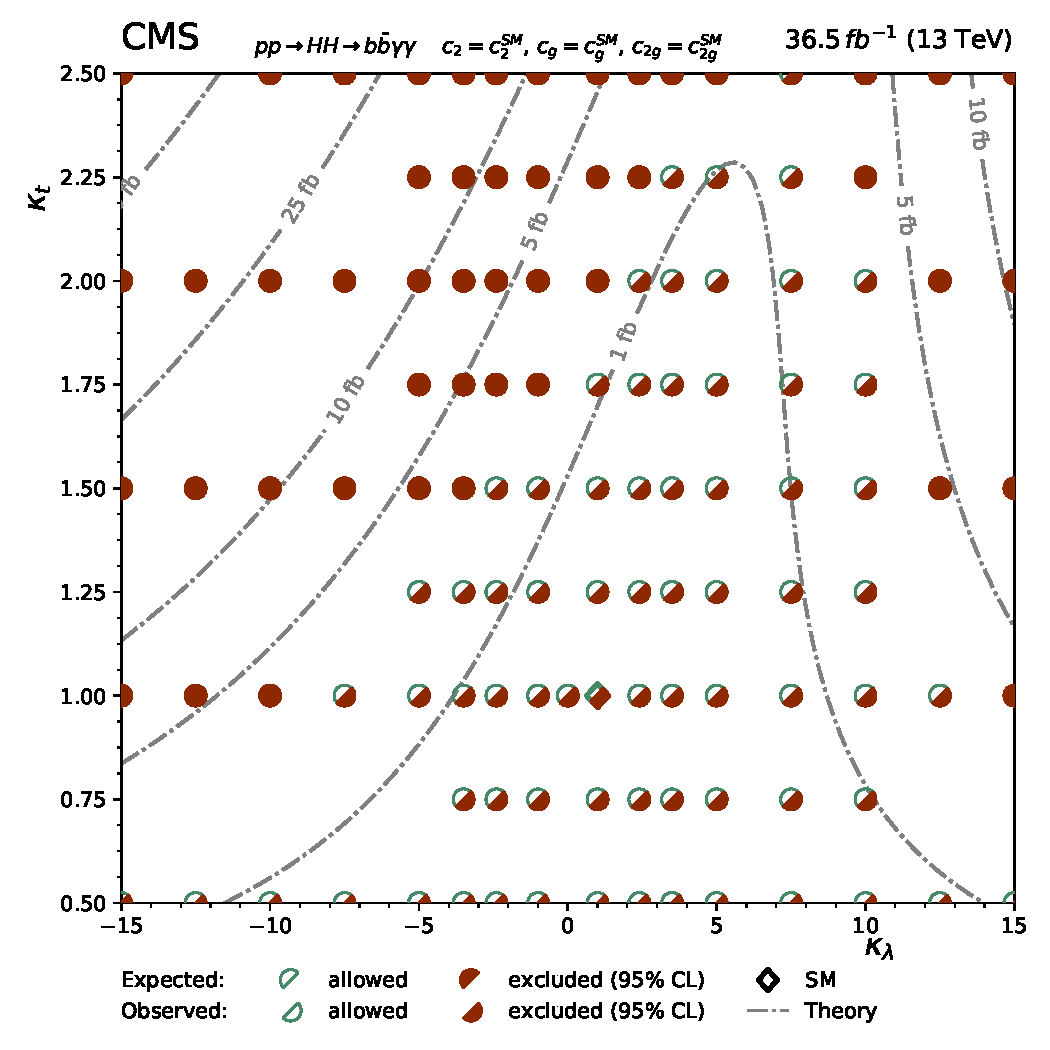
\includegraphics[width=0.7\textwidth]{NR_limits/NR_Limit_Lambda_Kt_Scan}\hfil
  \caption{Upper limits for the BSM models with varying
    $\kappa_\lambda-\kappa_t$ parameters, while other parameters are
    fixed to their SM values.}
  \label{fig:NRlim_2D}
\end{figure*}




%\begin{figure*}[h]
%  \centering
%  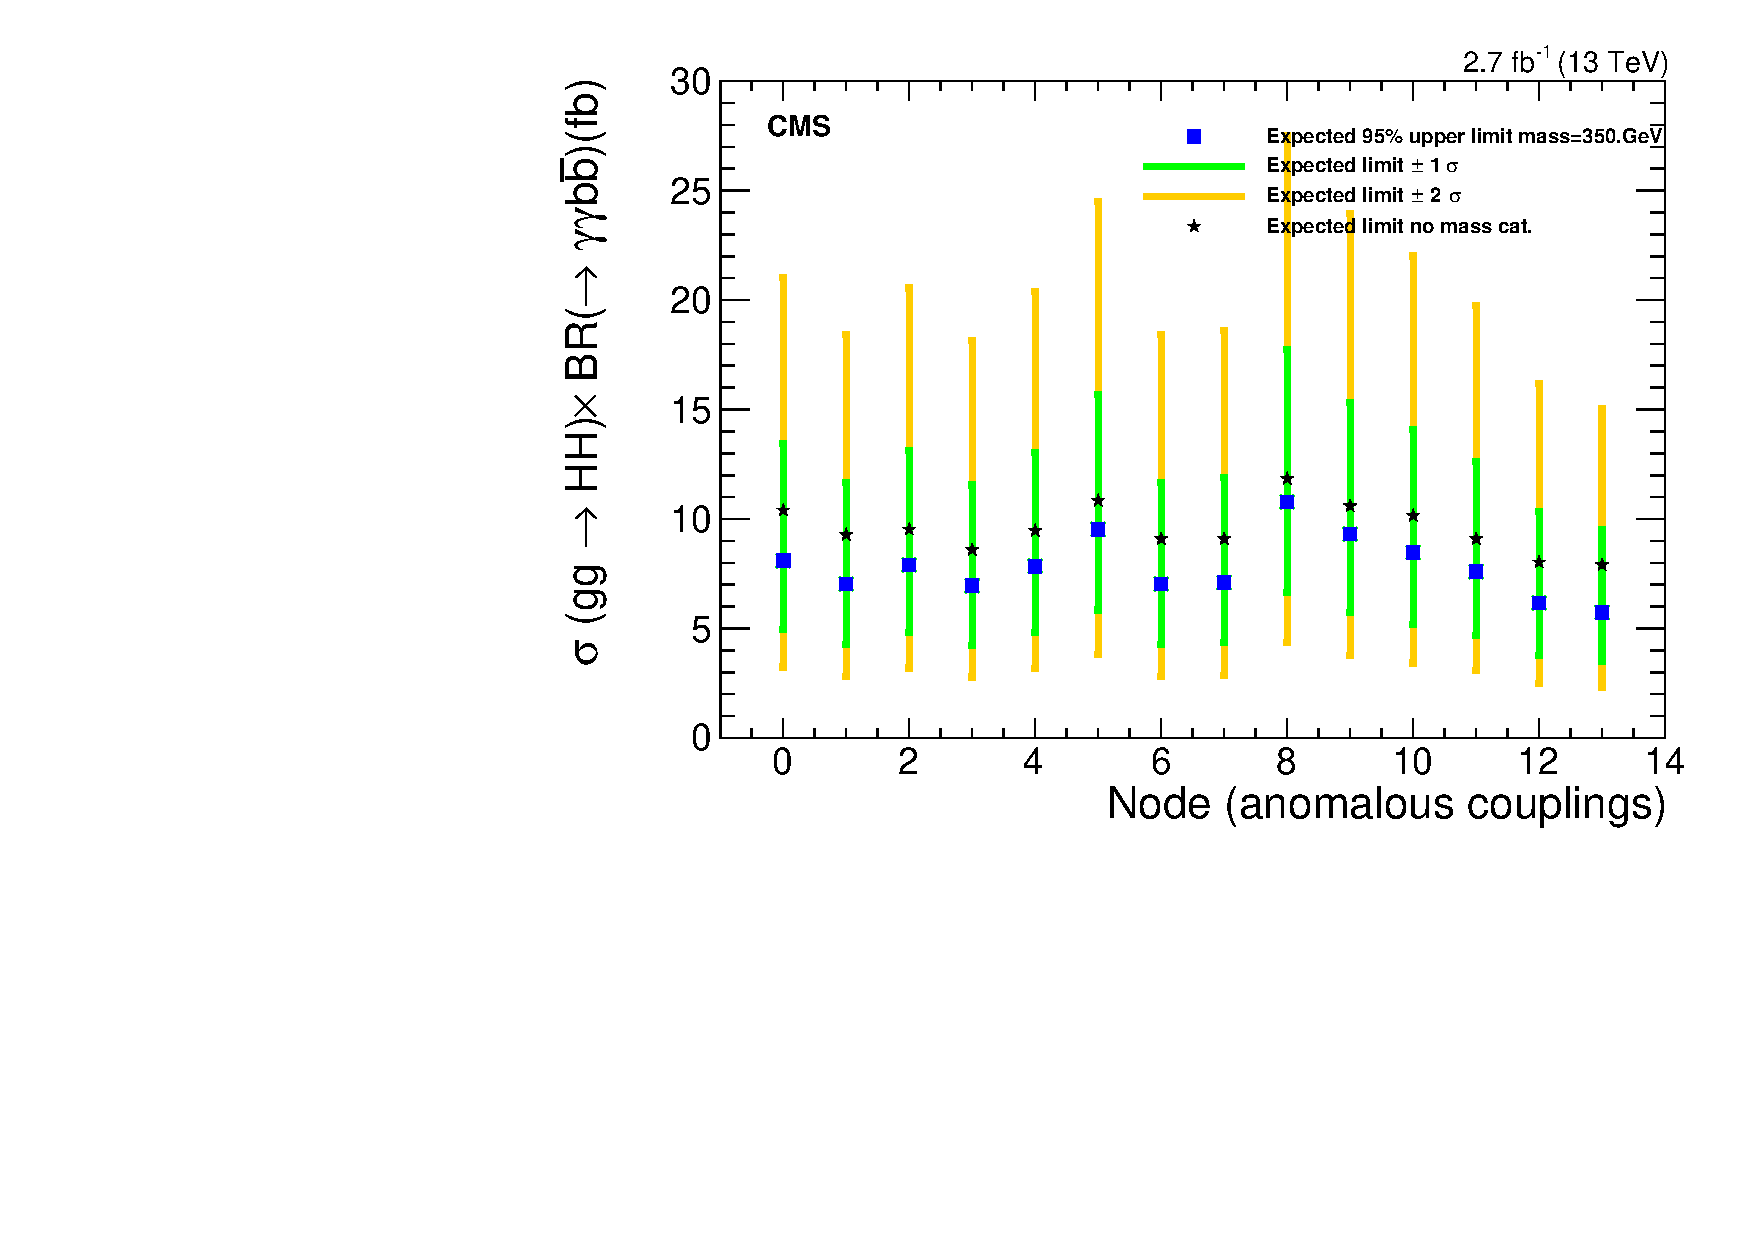
\includegraphics[width=0.55\textwidth]{Brazilian_NR_mass_350_PlusAll}\hfil
%  \caption{Four categories compared to two categories $95\%$ CL nonresonant expected upper limits  on the product~~\sigmaHH$\times$\ggbb~~for 14 different nodes described in subsection~\ref{sec:nonresMC} and in table~\ref{tab:bench}. The star markers are for no mass categorization. ERRATUM: This plot was made with a different version of the analysis, the study will be updated, but a similar conclusion is expected.}
%  \label{fig:BR_limits_PlusAll}
%\end{figure*}

%\begin{figure*}[h]
%  \centering
%  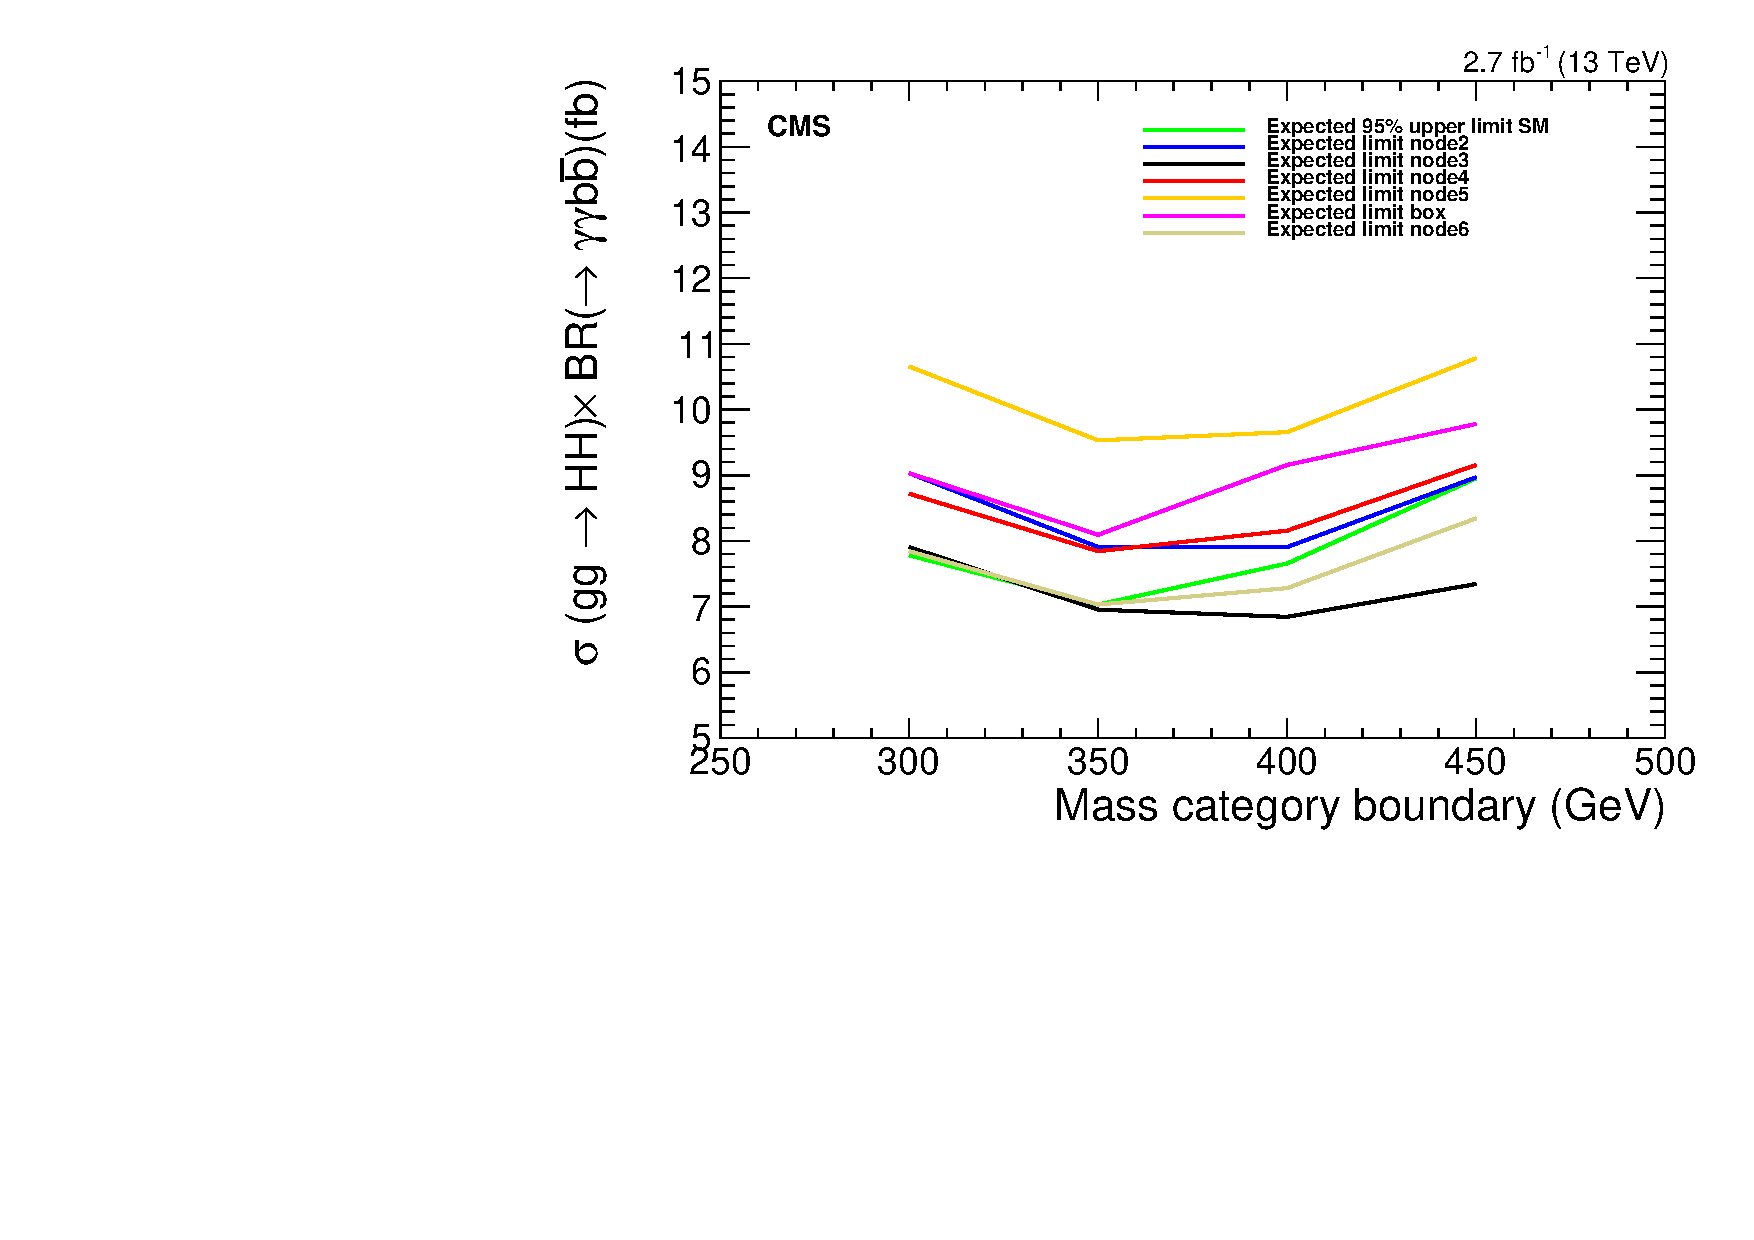
\includegraphics[width=0.55\textwidth]{NR_massScan_upTo_node6_Line}
%  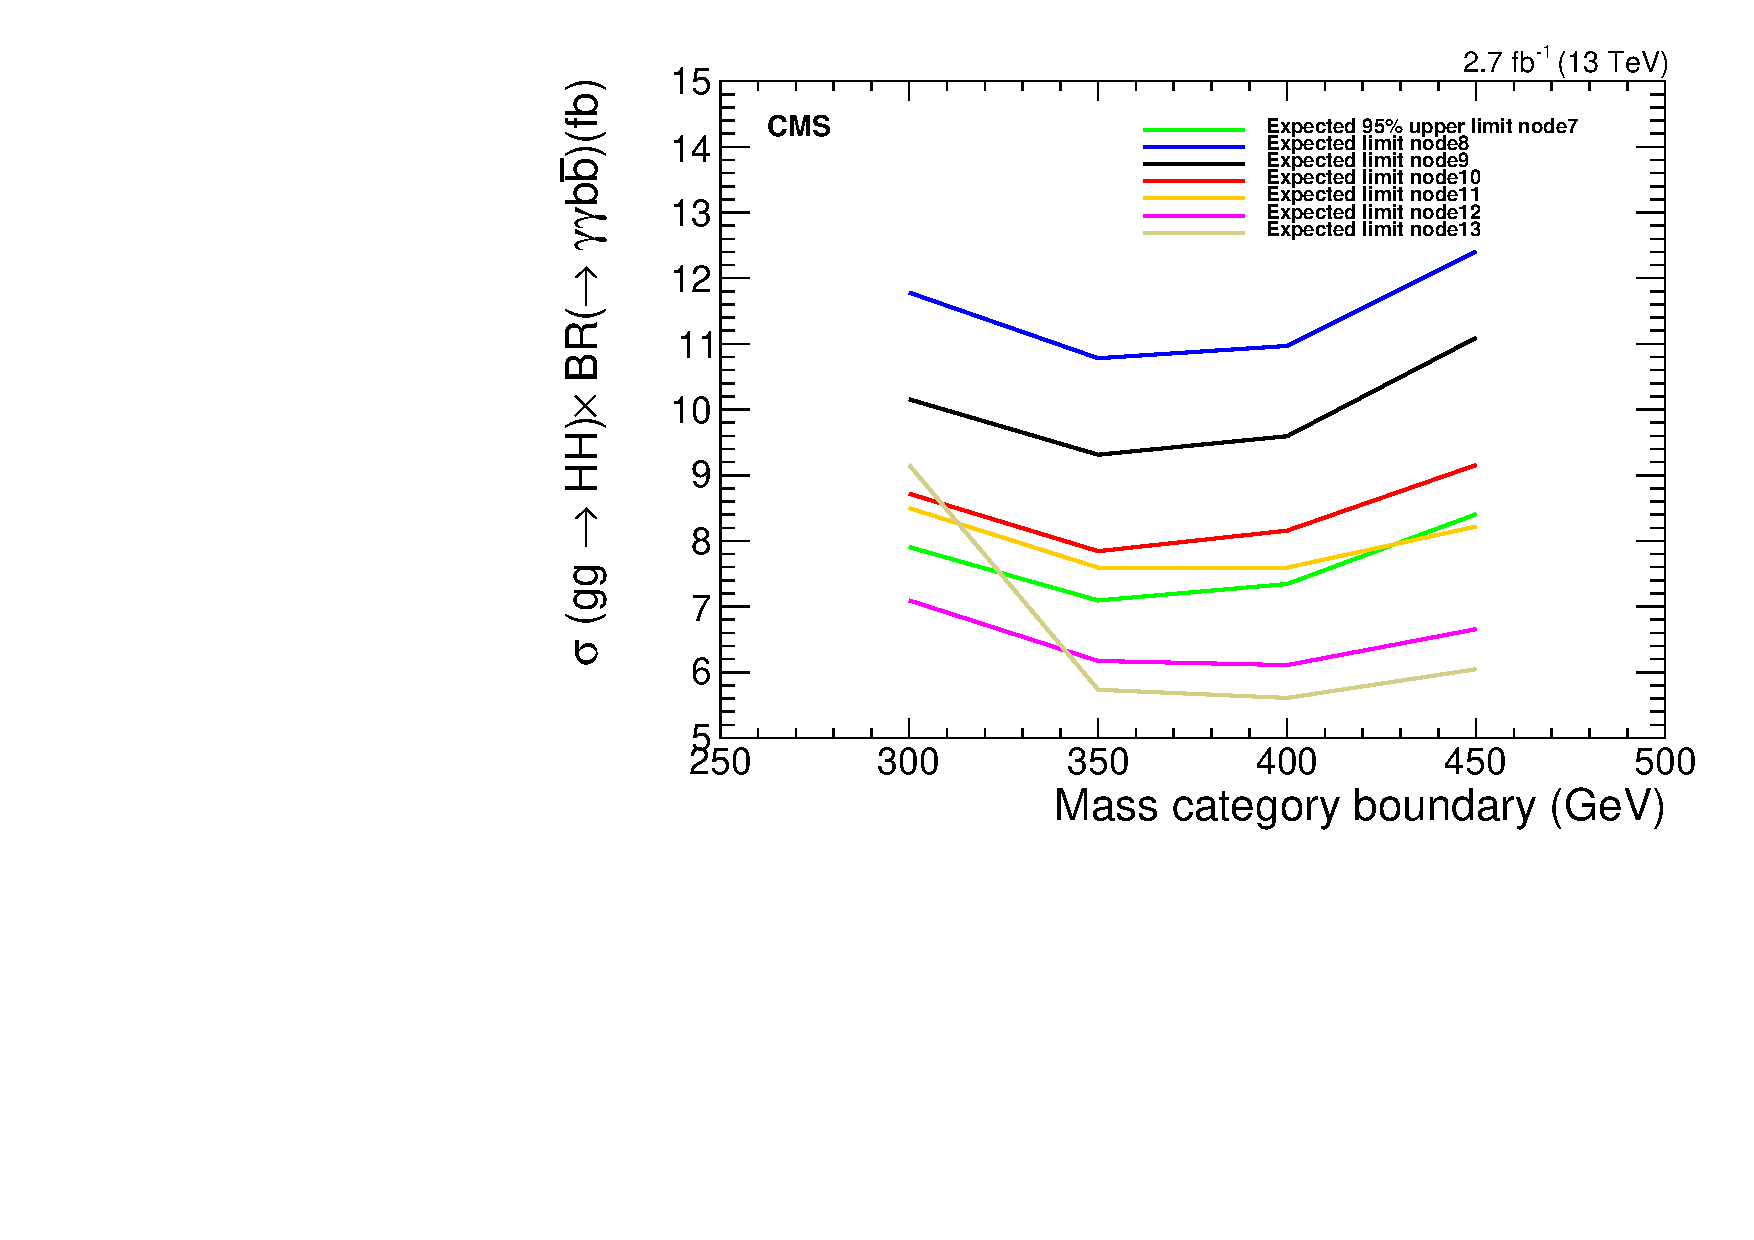
\includegraphics[width=0.55\textwidth]{NR_massScan_upTo_node13_Line}\hfil
%  \caption{Four categories mass scan for $95\%$ CL nonresonant expected upper limits on the product~~\sigmaHH$\times$\ggbb~~for  14 different nodes. (Top) for nodes up to node=6, (bottom) for nodes between node=7 and node=13. ERRATUM: This plot was made with a different version of the analysis, the study will be updated, but a similar conclusion is expected.}
%  \label{fig:BR_limits_mScan}
%\end{figure*}

%\begin{table}
%\centering
%\small{
%\begin{tabular}{|c||c|c|}
%\hline
%%Node & $95\%C.L. Limit $ &$m_{cat}$ improvement  \\\hline &  8.09 & 22.  \\
%%1  &  7.03  & 24.   \\ 
%2  &   7.91 & 17.        \\ 
%3  &  6.95 & 19.    \\
%4  &   7.84 & 17. \\ 
%5  &  9.53 & 12.    \\ 
%6  &   7.03 & 23.   \\ 
%7  &   7.09& 22.  \\ 
%8  &   10.78 & 9.     \\ 
%9  &  9.31 & 12.  \\ 
%10 &  8.47 & 17.    \\ 
%11 & 7.59 & 16.    \\ 
%12 &   6.17 & 23.    \\ 
%13 & 5.73 & 27.    \\ \hline
%\end{tabular}
%}
%\caption{\small The $95\%$ CL nonresonant upper limits  values when using  $m_{cat}=350. GeV$ categorization and the improvement expected when compared to limits with no mass categorization. ERRATUM: This table was made with a different version of the analysis, the study will be updated, but a similar conclusion is expected.\label{tab:mcat}}
%\end{table} 
